\documentclass{article}
\usepackage{amsmath}
\usepackage{amssymb}
\usepackage{graphicx}
\usepackage{hyperref}
\usepackage[version=4]{mhchem}


\begin{document}
\section*{Problem}
\(A B\) is the diameter of circle \(O\). \(C\) is a point on the circumference. \(P\) is a point on the circumference \(P F\) is perpendicular to \(A B\). \(P F\) meets \(A C\) at \(E, A B\) at \(D\) and the extension of \(B C\) at \(F\). Show that \(D P^{2}=D E \cdot D F\).\\
\centering
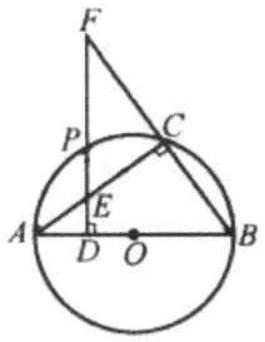
\includegraphics[width=\textwidth]{images/170(2).jpg}

\section*{Solution}
Connect \(P A\) and \(P B . A B\) is the hypotenuse of right triangles \(A P B\) and \(A C B\), so \(\angle A P B=90^{\circ}\) and \(\angle A C B=90^{\circ}\).\\
Since triangle \(A P B\) is a right triangle, \(D P^{2}=A D \cdot D B\).\\
Instead of showing that \(D P^{2}=D E \cdot D F\), we can now prove that \(A D \cdot D B=D E \cdot D F\).\\
Note that \(\triangle A D E \sim \triangle F D B\).\\
We know that \(\angle F=\angle E A D\), and \(\angle A D E=\angle F D B=90^{\circ}\).\\
\centering
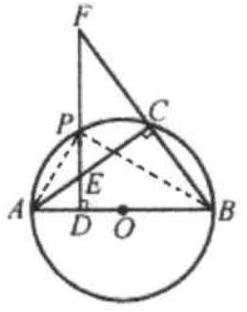
\includegraphics[width=\textwidth]{images/173(1).jpg}

Therefore \(\triangle A D E \sim \triangle F D B \Rightarrow \frac{A D}{D E}=\frac{D F}{D B} \Rightarrow\) \(A D \cdot D B=D E \cdot D F\).

\end{document}
